\documentclass[11pt]{article}

\usepackage[a4paper,margin=24mm]{geometry}
\usepackage{xcolor}
\usepackage{listings}
\usepackage[most]{tcolorbox}
\usepackage{booktabs}
\usepackage{array}
\usepackage{hyperref}
\usepackage{luanumbers}

\LuaNumbersSetup{
  decimals=1,
  rounding=half-up,
  pad-zeroes=true,
  integers=false,
  warnings=once
}

\definecolor{codebackground}{HTML}{F5F7FA}
\definecolor{codeframe}{HTML}{CBD5E1}
\definecolor{codekeyword}{HTML}{1D4ED8}
\definecolor{codecomment}{HTML}{64748B}
\definecolor{outputbackground}{HTML}{F0FDF4}
\definecolor{outputframe}{HTML}{16A34A}
\definecolor{warningbackground}{HTML}{FFF7ED}
\definecolor{warningframe}{HTML}{EA580C}

\lstdefinestyle{latexinput}{
  language=[LaTeX]TeX,
  basicstyle=\ttfamily\small,
  keywordstyle=\color{codekeyword}\bfseries,
  commentstyle=\color{codecomment}\itshape,
  backgroundcolor=\color{codebackground},
  frame=single,
  rulecolor=\color{codeframe},
  numbers=left,
  numberstyle=\scriptsize\color{codecomment},
  numbersep=10pt,
  breaklines=true,
  columns=fullflexible,
  keepspaces=true,
  showstringspaces=false,
  xleftmargin=4pt,
  framexleftmargin=4pt
}

\newtcolorbox{processedoutput}{
  title=Processed output,
  colback=outputbackground,
  colframe=outputframe,
  coltitle=white,
  fonttitle=\bfseries,
  boxrule=0.8pt,
  arc=2pt
}

\newtcolorbox{importantnote}{
  title=Important,
  colback=warningbackground,
  colframe=warningframe,
  coltitle=white,
  fonttitle=\bfseries,
  boxrule=0.8pt,
  arc=2pt
}

\newcommand\InputHeading{\par\smallskip\noindent\textbf{LaTeX input}\par\smallskip}
\newcolumntype{L}[1]{>{\raggedright\arraybackslash}p{#1}}

\title{The \texttt{luanumbers} Package\\\large Document-Wide Decimal Adjustment from a Single Preamble Setup}
\author{Parsa Yazdi\\\small Developer and maintainer}
\date{Version 0.5.0, 10 June 2026}

\begin{document}
\maketitle

\section*{Summary}

\texttt{luanumbers} is a LuaLaTeX package that lets an author declare a
decimal-formatting policy once in the document preamble and apply it
automatically to ordinary decimal literals throughout prose and mathematics.
Existing numbers can remain in their natural LaTeX form: they do not normally
need to be wrapped individually in formatting commands, moved into special data
structures, or prepared with an additional number-formatting package. The Lua
implementation uses exact decimal-string arithmetic, preserves integers by
default, protects structural LaTeX data, and provides local exclusions for
selected sections, figures, tables, diagrams, and other objects. Explicit
formatting remains available for ambiguous or protected contexts where the
author's intent cannot be inferred safely. Documents using the package must be
compiled with LuaLaTeX.

\section*{Practical Advantages}

\begin{itemize}
  \item \textbf{One-time configuration:} precision, rounding mode, zero
    padding, and related behavior are declared together in the preamble.
  \item \textbf{Natural source text:} ordinary literals such as
    \texttt{3.14159} can be written directly instead of placing every value
    inside a dedicated formatting command.
  \item \textbf{Efficient document-wide revision:} changing one setup value
    can update the displayed precision across a long document without editing
    each occurrence manually.
  \item \textbf{Conservative automation:} integers, labels, references, file
    names, graphics coordinates, and ambiguous source are preserved according
    to documented safeguards.
  \item \textbf{Fine-grained control:} authors can exclude one selected object,
    protect recurring commands or environments, suspend processing temporarily,
    or request explicit formatting for an individual value.
  \item \textbf{Self-contained workflow:} the package supplies both the global
    automatic policy and the explicit per-value command, avoiding the need to
    combine separate number-rounding mechanisms for these tasks.
\end{itemize}

\clearpage
\tableofcontents

\section{Purpose and Requirements}

The \texttt{luanumbers} package is intended for documents whose decimal
precision should be controlled centrally. After one preamble setup, it adjusts
eligible decimal literals automatically across the document body. Authors can
therefore revise the document-wide precision without finding and rewriting
each number or marking every number with a special command. Exact
decimal-string arithmetic is used rather than binary floating point. The
package requires LuaLaTeX.

\begin{importantnote}
Automatic processing is intentionally conservative. Structural data, protected
commands, protected environments, URLs, versions, and other ambiguous values
are preserved. Use \verb|\LuaNumber| when formatting must be explicit.
\end{importantnote}

\section{Installation and Compilation}

Place \texttt{luanumbers.sty} and \texttt{luanumbers.lua} beside the document,
or install both files in a local TeX tree. Compile with:

\begin{lstlisting}[style=latexinput,language=bash,numbers=none]
lualatex document.tex
\end{lstlisting}

The package cannot be used with pdfLaTeX or XeLaTeX.

\section{Basic Setup}

\InputHeading
\LuaNumbersOff
\begin{lstlisting}[style=latexinput]
\usepackage{luanumbers}

\LuaNumbersSetup{
  decimals=1,
  rounding=half-up,
  pad-zeroes=true,
  integers=false,
  warnings=once
}
\end{lstlisting}
\LuaNumbersOn

With this configuration, decimal literals are shown with one decimal place,
while integers remain unchanged.

\section{Input and Output}

\InputHeading
\LuaNumbersOff
\begin{lstlisting}[style=latexinput]
Pi is approximately 3.14159265.
The measured value is 3.00 units.
The correction is -1.234 units.
There are 7 complete samples.
\end{lstlisting}
\LuaNumbersOn

\begin{processedoutput}
Pi is approximately 3.14159265.
The measured value is 3.00 units.
The correction is -1.234 units.
There are 7 complete samples.
\end{processedoutput}

The decimal values become \texttt{3.1}, \texttt{3.0}, and \texttt{-1.2}.
The integer \texttt{7} is not changed.

\subsection{Mathematics}

\InputHeading
\LuaNumbersOff
\begin{lstlisting}[style=latexinput]
\[
  1.23456 + 9.87654 = 11.11110
\]
\end{lstlisting}
\LuaNumbersOn

\begin{processedoutput}
\[
  1.23456 + 9.87654 = 11.11110
\]
\end{processedoutput}

\subsection{Scientific Notation}

Scientific notation is preserved by default. Thus \texttt{6.022e2} becomes
\texttt{6.0e2} with the one-decimal setup. A literal such as \texttt{6e2} is
unchanged when \texttt{integers=false}.

\subsection{Explicit Formatting}

\verb|\LuaNumber| always formats its argument using the active settings:

\begin{lstlisting}[style=latexinput]
The result is \LuaNumber{12.3456}.
\end{lstlisting}

It is also the preferred command for values in ambiguous contexts or protected
environments.

\section{Configuration Reference}

\begin{center}
\begin{tabular}{@{}lll@{}}
\toprule
Setting & Default & Accepted values \\
\midrule
\texttt{decimals} & \texttt{2} & Integer from 0 to 100 \\
\texttt{rounding} & \texttt{half-up} & \texttt{half-up}, \texttt{half-even}, \texttt{truncate}, \texttt{floor}, \texttt{ceil} \\
\texttt{pad-zeroes} & \texttt{true} & Boolean \\
\texttt{integers} & \texttt{false} & Boolean \\
\texttt{preserve-exponent} & \texttt{true} & Boolean \\
\texttt{normalize-negative-zero} & \texttt{true} & Boolean \\
\texttt{input-decimal} & \texttt{dot} & \texttt{dot}, \texttt{comma}, \texttt{both} \\
\texttt{auto-protect} & \texttt{true} & Boolean \\
\texttt{warnings} & \texttt{once} & \texttt{off}, \texttt{once}, \texttt{all}, \texttt{error} \\
\bottomrule
\end{tabular}
\end{center}

\subsection{Rounding Modes}

\texttt{half-up} rounds a decimal tie away from zero. \texttt{half-even}
rounds a tie toward an even final digit. \texttt{truncate} discards excess
digits. \texttt{floor} rounds toward negative infinity and \texttt{ceil}
rounds toward positive infinity.

\section{Exact Decimal Arithmetic}

The formatter operates on digit strings. It therefore handles values such as
\texttt{2.675}, very large decimal strings, and halfway cases without first
converting them to a Lua floating-point number. It also supports leading
decimals such as \texttt{.125}, decimal commas when configured, Unicode minus
signs, and negative-zero normalization.

Automatic mode does not interpret a trailing form such as \texttt{3.} because
it is indistinguishable from sentence punctuation. The explicit command
\verb|\LuaNumber{3.}| can format that form safely.

\section{Local Object Exclusion}

The recommended way to preserve one particular object is the built-in
\texttt{luanumbersexclude} environment. Only source inside that specific
wrapper is excluded. Other sections, figures, tables, and objects of the same
type continue to use automatic rounding.

The wrapper can contain the object's heading, caption, label, body, and nested
environments. All numeric source within it is copied to TeX unchanged.
Generated metadata files such as \texttt{.aux}, \texttt{.toc}, \texttt{.lof},
and \texttt{.lot} are never rewritten, so protected headings and labels remain
stable across repeated LaTeX passes.

\subsection{One Selected Section}

\begin{lstlisting}[style=latexinput]
\begin{luanumbersexclude}
\section{Experimental results 3.14159}
\label{sec:results-3.14159}

This selected section preserves 3.14159 exactly.
\end{luanumbersexclude}

\section{Discussion 3.14159}
This later section is processed normally: 3.14159.
\end{lstlisting}

The first heading, label, and section body are preserved. The second section
is outside the wrapper, so its decimal literals use the configured precision.
The exclusion ends exactly at \verb|\end{luanumbersexclude}|; it does not alter
all other section commands.

\subsection{One Selected Figure}

\begin{lstlisting}[style=latexinput]
\begin{luanumbersexclude}
\begin{figure}
  \centering
  \includegraphics[width=0.75\textwidth]{result-3.14159.pdf}
  \caption{Unmodified measurement 3.14159}
  \label{fig:result-3.14159}
\end{figure}
\end{luanumbersexclude}
\end{lstlisting}

Only this figure is isolated. Its graphics options, file name, caption, label,
and body remain unchanged. A later figure outside the wrapper is unaffected by
this exclusion policy.

\subsection{One Selected Table}

\begin{lstlisting}[style=latexinput]
\begin{luanumbersexclude}
\begin{table}
  \centering
  \caption{Raw values from dataset 2.7}
  \label{tab:raw-2.7}
  \begin{tabular}{cc}
    1.2345 & 9.8765 \\
  \end{tabular}
\end{table}
\end{luanumbersexclude}
\end{lstlisting}

This preserves the selected table's data and metadata without disabling
automatic rounding in other tables.

\begin{importantnote}
The \verb|\label| command is protected by default even without a local wrapper,
so label keys such as \texttt{fig:result-3.14159} are not rewritten. The local
wrapper additionally preserves the selected object's visible caption, heading,
body, and other numeric source.
\end{importantnote}

\section{Globally Protected Environment Types}

The package protects these environments by default:

\begin{center}
\texttt{tikzpicture}, \texttt{axis}, \texttt{pgfpicture},
\texttt{verbatim}, \texttt{verbatim*}, \texttt{lstlisting},
\texttt{minted}, \texttt{filecontents}, and \texttt{filecontents*}.
\end{center}

All numeric source inside a protected environment is passed through unchanged.
For graphics environments, this refers only to the package's \emph{automatic
input rewriting}. The explicit \verb|\LuaNumber{...}| command still works
inside a protected environment because TeX executes that command after the
input line has been preserved. This distinction prevents coordinates and data
from being changed while still allowing selected visible labels to be rounded.
Register one environment or a comma-separated list in the preamble only when
\emph{every instance} of that environment type should be excluded:

\begin{lstlisting}[style=latexinput]
\LuaNumbersProtectEnvironment{mydiagram}

\LuaNumbersProtectEnvironments{
  mydiagram
}
\end{lstlisting}

Remove protection with the corresponding singular or plural command:

\begin{lstlisting}[style=latexinput]
\LuaNumbersUnprotectEnvironment{mydiagram}
\LuaNumbersUnprotectEnvironments{mydiagram,otherdiagram}
\end{lstlisting}

\begin{importantnote}
Registering \texttt{figure} or \texttt{table} here is global: every matching
float in the document is preserved. To isolate one particular figure or table,
use \texttt{luanumbersexclude} around that object instead.
\end{importantnote}

\section{Protected Commands}

Arguments of common structural commands are protected by default, including
references, citations, URLs, file names, graphics options, length settings,
and TikZ/PGF setup commands.

Document-specific commands can be registered in the preamble when every use of
that command should have protected arguments:

\begin{lstlisting}[style=latexinput]
\LuaNumbersProtectCommands{
  caption,
  custommetadata
}
\end{lstlisting}

This applies globally to every registered command. Use the local
\texttt{luanumbersexclude} wrapper to preserve only one particular section or
caption. Command names may be written with or without their leading backslash.
Multiline braced arguments are tracked until their closing brace.

The related singular and removal operations are:

\begin{lstlisting}[style=latexinput,numbers=none]
\LuaNumbersProtectCommand{command}
\LuaNumbersUnprotectCommand{command}
\LuaNumbersUnprotectCommands{command-a,command-b}
\end{lstlisting}

\section{TikZ, PGFPlots, and Beamer}

The package does \emph{not} automatically rewrite numeric literals inside
\texttt{tikzpicture}, \texttt{pgfpicture}, or \texttt{axis}. This is deliberate:
the same literal may be a coordinate, dimension, transformation, plot datum, or
style parameter, and rounding it could alter the graphic rather than merely its
printed text.

The resulting behavior is:

\LuaNumbersOff
\begin{center}
\begin{tabular}{@{}L{0.42\linewidth}L{0.18\linewidth}L{0.29\linewidth}@{}}
\toprule
Source context & Automatic rounding & Recommended control \\
\midrule
Ordinary text outside graphics & Yes & \texttt{\string\LuaNumbersSetup} \\
TikZ coordinates and dimensions & No & Leave protected \\
Plain numeric text in a TikZ node & No & Use \texttt{\string\LuaNumber} \\
PGFPlots coordinates and tables & No & Leave protected \\
PGFPlots-generated tick labels & No & Use PGFPlots number formatting \\
\bottomrule
\end{tabular}
\end{center}
\LuaNumbersOn

Explicit \verb|\LuaNumber| calls are still processed inside protected graphics
environments. For example, the geometry below is copied unchanged, but the
visible value in the node is rounded to the package precision:

\begin{lstlisting}[style=latexinput]
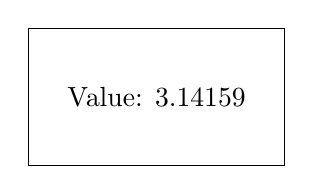
\begin{tikzpicture}
  \draw (0.00,0.00) rectangle (3.26,1.74);
  \node at (1.63,0.87)
    {Value: \LuaNumber{3.14159}};
\end{tikzpicture}
\end{lstlisting}

\LuaNumbersOff
Thus, with one decimal place, \texttt{(3.26,1.74)} remains exactly a TikZ
coordinate while the node displays \texttt{Value: 3.1}. A plain node such as
\verb|\node {Value: 3.14159};| would retain \texttt{3.14159}, because it has not
requested explicit formatting.
\LuaNumbersOn

PGFPlots creates tick labels from plot data after reading the source. Configure
those labels through PGFPlots rather than by changing the underlying data:

\begin{lstlisting}[style=latexinput]
\pgfplotsset{
  tick label style={/pgf/number format/.cd,
    fixed, fixed zerofill, precision=1}
}
\end{lstlisting}

It is possible to opt into automatic source rewriting globally:

\begin{lstlisting}[style=latexinput]
\LuaNumbersUnprotectEnvironment{tikzpicture}
\LuaNumbersUnprotectEnvironment{axis}
\end{lstlisting}

This affects every numeric literal in every matching environment, including
coordinates and dimensions, so it is not the recommended method for formatting
displayed labels.

The same behavior works when TikZ is nested inside a Beamer frame. Ordinary
frame text remains subject to automatic rounding, while the graphics source is
preserved and explicit \verb|\LuaNumber| calls inside the graphic still work.

\section{Warnings and Ambiguous Input}

Automatic mode leaves suspicious values unchanged and issues a warning when a
number appears in a context resembling a URL, date, ratio, key-value setting,
grouped number, or version. Examples include:

\LuaNumbersOff
\begin{lstlisting}[style=latexinput,numbers=none]
https://host/3.14159
key=3.14159
1,234.56
1.2.3
\end{lstlisting}
\LuaNumbersOn

Set \texttt{warnings=error} during validation or continuous integration to stop
compilation whenever such a case requires review. Use \verb|\LuaNumber| when
the suspicious value is definitely display text.

\section{Manual Suspension}

Automatic processing can be suspended for exceptional source regions:

\begin{lstlisting}[style=latexinput]
\LuaNumbersOff
This value is preserved exactly: 3.14159265.
\LuaNumbersOn
\end{lstlisting}

Place these commands on separate source lines. Registered environment and
command protection is preferable for recurring structures, while
\texttt{luanumbersexclude} is preferable for one selected document object.

\section{Limitations}

The package processes LuaTeX input lines before TeX expands macros. It cannot
infer semantic intent from arbitrary macro-generated source, numbers assembled
from several macros, or environments whose begin/end commands are generated
indirectly. Automatic processing is therefore a convenience layer, while
\verb|\LuaNumber| remains the deterministic interface.

When \texttt{integers=true}, integer arguments expected by LaTeX commands may
be converted to decimal strings. Use that setting cautiously and protect
structural commands that require literal integers.

\section{Development and Verification}

From the project root:

\begin{lstlisting}[style=latexinput,language=bash,numbers=none]
make doc          # build this manual
make examples     # build TikZ/PGFPlots and Beamer examples
make test         # run Lua assertions and compile the smoke test
make clean        # remove generated TeX files
\end{lstlisting}

\end{document}
